\documentclass[border=5pt]{standalone}
\usepackage{pgfplots}
\usepgfplotslibrary{groupplots}
\pgfplotsset{compat=1.18}

\definecolor{sourceblue}{HTML}{2166AC}
\definecolor{targetorange}{HTML}{D6604D}
\definecolor{cleanblue}{HTML}{92C5DE}
\definecolor{patchedgreen}{HTML}{4D9221}

\begin{document}
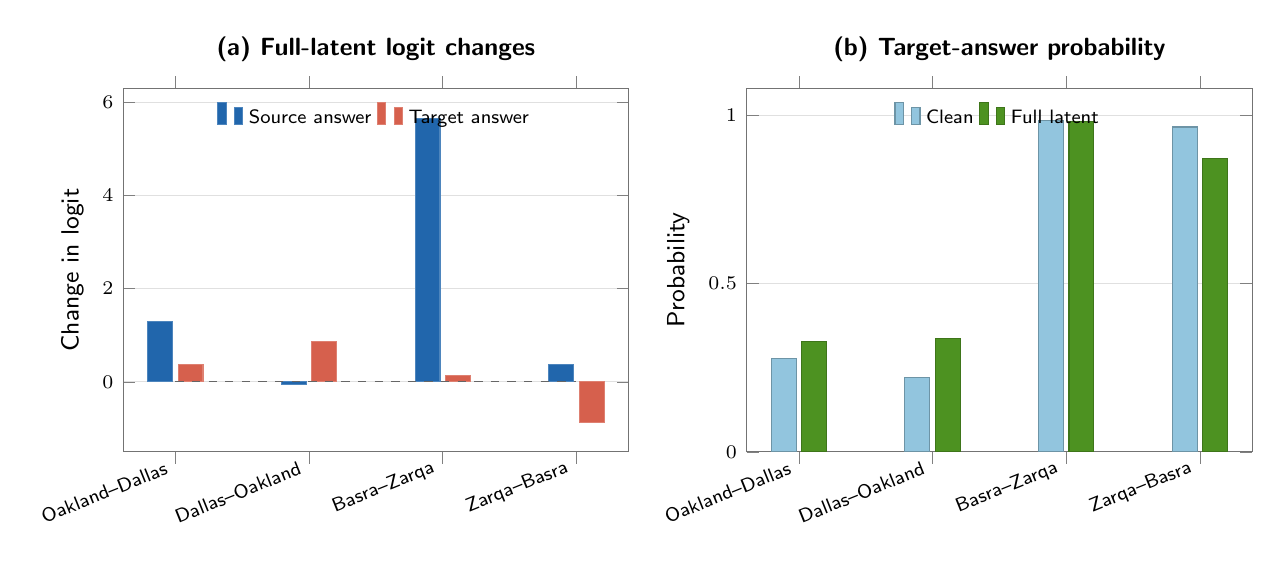
\begin{tikzpicture}
\begin{groupplot}[
    group style={group size=2 by 1, horizontal sep=1.5cm},
    width=8.0cm,
    height=6.2cm,
    ymajorgrids,
    grid style={draw=black!12},
    axis line style={draw=black!55},
    tick label style={font=\sffamily\scriptsize},
    label style={font=\sffamily\small},
    title style={font=\sffamily\small\bfseries},
    legend style={font=\sffamily\scriptsize, draw=none, fill=none},
    symbolic x coords={OtoD,DtoO,BtoZ,ZtoB},
    xtick=data,
    xticklabels={Oakland--Dallas,Dallas--Oakland,Basra--Zarqa,Zarqa--Basra},
    x tick label style={rotate=22,anchor=east},
    enlarge x limits=0.13,
]

\nextgroupplot[
    title={(a) Full-latent logit changes},
    ybar=2pt,
    bar width=9pt,
    ymin=-1.5,
    ymax=6.3,
    ylabel={Change in logit},
    legend columns=2,
    legend style={at={(0.5,0.98)},anchor=north},
]
\addplot+[fill=sourceblue, draw=sourceblue!80] coordinates {
    (OtoD,1.30) (DtoO,-0.06) (BtoZ,5.65) (ZtoB,0.38)
};
\addlegendentry{Source answer}
\addplot+[fill=targetorange, draw=targetorange!80] coordinates {
    (OtoD,0.38) (DtoO,0.87) (BtoZ,0.13) (ZtoB,-0.88)
};
\addlegendentry{Target answer}
\draw[black!60, dashed] (axis cs:OtoD,0) -- (axis cs:ZtoB,0);

\nextgroupplot[
    title={(b) Target-answer probability},
    ybar=2pt,
    bar width=9pt,
    ymin=0,
    ymax=1.08,
    ylabel={Probability},
    legend columns=2,
    legend style={at={(0.5,0.98)},anchor=north},
]
\addplot+[fill=cleanblue, draw=cleanblue!75!black] coordinates {
    (OtoD,0.2773) (DtoO,0.2217) (BtoZ,0.9844) (ZtoB,0.9648)
};
\addlegendentry{Clean}
\addplot+[fill=patchedgreen, draw=patchedgreen!80!black] coordinates {
    (OtoD,0.3281) (DtoO,0.3359) (BtoZ,0.9805) (ZtoB,0.8711)
};
\addlegendentry{Full latent}

\end{groupplot}
\end{tikzpicture}
\end{document}
